\chapter{Competitive Programming Problems}
\section{Common function functions }
This section describes the utility functions that are used to write solution for the followings problems.

\begin{lstlisting}[language=c++, caption="For each functions"]

template <typename Iterator, typename Lambda>
void for_each(Iterator s, Iterator e, Lambda l) {
  while (s != e) {
    l(*s);
    s++;
  }
}

//Lambda has type (T& -> int -> void)
template <typename Container, typename Lambda>
void for_each_i(Container& v, const int s, const int e, Lambda l) {
    int i=s;
    while (i < e){
        l(v[i],i);
        i++;
    }
}
	\end{lstlisting}
	
	
	
\begin{lstlisting}[language=c++, caption="Store credit c++ solution"]

template <typename T, typename Iterator>
bool contains(const Iterator s, const Iterator e, const T& value) {
  auto predicate_equal = [&](T curr) { return value == curr; };
  bool ret = e == find_if(s, e, predicate_equal);
  return !ret;
}

// Return value
// Iterator to the first element satisfying the condition or last if no such
// element is found.
template <typename Iterator, typename Lambda>
Iterator find_if(Iterator s, Iterator e, Lambda predicate) {
  while (s != e) {
    if (predicate(*s))
      return s;

    s++;
  }
  return e;
}

// Return value
// Iterator to the first element satisfying the condition or last if no such
// element is found.
template <typename Iterator, typename Lambda>
inline Iterator find_if_not(Iterator s, Iterator e, Lambda predicate) {
  auto not_predicate = [&](auto v) { return !predicate(v); };
  return find_if(s, e, not_predicate);
}

	\end{lstlisting}



\begin{lstlisting}[language=c++, caption="Store credit c++ solution"]
template <typename Iterator, typename Lambda>
bool all_of(Iterator s, Iterator e, Lambda predicate) {
  while (s != e) {
    if (!predicate(*s))
      return false;
    s++;
  }
  return true;
}

template <typename Iterator, typename Lambda>
bool any_of(Iterator s, Iterator e, Lambda predicate) {
  while (s != e) {
    if (predicate(*s))
      return true;
    s++;
  }

  return false;
}
\end{lstlisting}





\begin{lstlisting}[language=c++, caption="Store credit c++ solution"]
// Lambda has type: D -> T -> D
template <typename D, typename Iterator, typename Lambda>
D fold(Iterator s, Iterator e, const D& a, Lambda l) {
  D acc = a;
  while (s != e) {
    acc = l(acc, *s);
    s++;
  }
  return acc;
}

\end{lstlisting}


\begin{lstlisting}[language=c++, caption="Read input functions"]
template <typename T>
void readVector(std::vector<T>& v, const int size, std::istream& is=std::cin) {
  LOOPUP(i, size) {
    T a;
    is >> a;
    v.push_back(a);
  }
}

template <typename T, unsigned int D>
void readArray(std::array<T, D>& v, std::istream& is=std::cin) {
  LOOPUP(i, D) {
    T a;
    is>> a;
    v[i] = a;
  }
}


void read(auto& v, const unsigned int size, std::istream& is=std::cin) {
    using T=typename std::remove_reference<decltype(v[0])>::type;
  LOOPUP(i, size) {
    T a;
    is>> a;
    v[i] = a;
  }
}
\end{lstlisting}


\begin{lstlisting}[language=c++, caption="Store credit c++ solution"]
template<typename T>
inline T safe_midpoint(const T lo, const T hi){
    return lo+(hi-lo)/2;
}


template<typename T>
inline T unsafe_midpoint(const T lo, const T hi){
    return (hi+lo)/2;
}


template<typename T>
inline bool lt(const T& v1,const T& v2){
    return v1 < v2;
}

template<typename T>
inline bool eq(const T& v1,const T& v2){
    return v1 == v2;
}

template<typename T>
inline bool gt(const T& v1,const T& v2){
    return v1 > v2;
}

template<typename T>
inline bool gte(const T& v1,const T& v2){
    return gt(v1,v2) || eq (v1,v2);
}
template<typename T>
inline bool lte(const T& v1,const T& v2){
    return lt<T>(v1,v2) || eq<T>(v1,v2);
}

\end{lstlisting}




\begin{problem}{\textit{Store Credit} - \textbf{Google Jam Qualification Round Africa 2010}}
You receive a credit C at a local store and would like to buy two items. You first walk through the store and create a list L of all available items. From this list you would like to buy two items that add up to the entire value of the credit. The solution you provide will consist of the two integers indicating the positions of the items in your list (smaller number first).

\textbf{Input}

The first line of input gives the number of cases, N. N test cases follow. For each test case there will be:
One line containing the value C, the amount of credit you have at the store.
One line containing the value I, the number of items in the store.
One line containing a space separated list of I integers. Each integer P indicates the price of an item in the store. Each test case will have exactly one solution.

\textbf{Output}

For each test case, output one line containing "Case \#x: " followed by the indices of the two items whose price adds up to the store credit. The lower index should be output first.
\begin{framed}
	\begin{verbatim}
Input 
3
100
3
5 75 25
200
7
150 24 79 50 88 345 3
8
8
2 1 9 4 4 56 90 3

Output 
Case #1: 2 3
Case #2: 1 4
Case #3: 4 5
	\end{verbatim}
\end{framed}

\end{problem}

\begin{solution}
	
	\begin{lstlisting}[language=c++, caption="Store credit c++ solution"]

#include<common.h>
using namespace std;

int main(){
    using P=pair<int,int>;
    int N; cin>>N;

    LOOPUP(i,N){
        int C; cin>>C;
        int I; cin>>I;
        vector<int> items(I);
        vector<P> ip(I);
        DS::read(items,I);
        DS::for_each_i(ip,0,I,
            [&](auto& el, const int idx){el.first=items[idx]; el.second=idx;}
        );

        DS::quicksort(ip,0,I,DS::lt<P>);
        auto eq_fn = [](const P& p, const int v){ return p.first==v; };
        auto cmp_fn = [](const P& p, const int v){ return p.first<v; };
        LOOPUP(j,ip.size()){
            int val = (C-items[j]);
            int idx = DS::binary_search_idx(ip,0,ip.size(), val ,eq_fn,cmp_fn);
            //found. pickup the one with lowest INDEX
            if(idx!= -1){
                int retidx =idx;
                bool good=false;//check we do not pickup the same element twice
                while(eq_fn(ip[retidx],val) && j!= ip[retidx].second ){
                    retidx--;
                    good=true;
                }
                if(good){
                    int l = j+ 1;
                    int h = ip[retidx+1].second+1;
                    cout<<"Case #"<<i+1<<": "<<min(l,h)<<" "<<max(l,h)<<endl;
                    int sum = items[j] + items[ip[retidx+1].second];
                    assert(sum==C);
                    break;
                }
            }
        }
    }//foreach testcase
    return 0;
}

	\end{lstlisting}
\end{solution}





\begin{problem}{\textit{Rope Intranet} - \textbf{Google Jam Round 1C 2010}}

A company is located in two very tall buildings. The company intranet connecting the buildings consists of many wires, each connecting a window on the first building to a window on the second building.

You are looking at those buildings from the side, so that one of the buildings is to the left and one is to the right. The windows on the left building are seen as points on its right wall, and the windows on the right building are seen as points on its left wall. Wires are straight segments connecting a window on the left building to a window on the right building.

You've noticed that no two wires share an endpoint (in other words, there's at most one wire going out of each window). However, from your viewpoint, some of the wires intersect midway. You've also noticed that exactly two wires meet at each intersection point.

On the above picture, the intersection points are the black circles, while the windows are the white circles.

How many intersection points do you see?

\begin{figure}
\centering
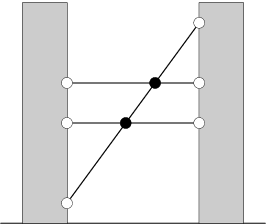
\includegraphics[scale=1]{ropeinternet}
\caption{}
\label{fig:ropeinternet}
\end{figure}

You've noticed that no two wires share an endpoint (in other words, there's at most one wire going out of each window). However, from your viewpoint, some of the wires intersect midway. You've also noticed that exactly two wires meet at each intersection point.

On figure \ref{fig:ropeinternet}, the intersection points are the black circles, while the windows are the white circles.

How many intersection points do you see?



\textbf{Input}
The first line of the input gives the number of test cases, T. T test cases follow. Each case begins with a line containing an integer N, denoting the number of wires you see.

The next N lines each describe one wire with two integers Ai and Bi. These describe the windows that this wire connects: Ai is the height of the window on the left building, and Bi is the height of the window on the right building.


\textbf{Output}
For each test case, output one line containing "Case \#x: y", where x is the case number (starting from 1) and y is the number of intersection points you see.

\begin{framed}
	\begin{verbatim}
Input 
2
3
1 10
5 5
7 7
2
1 1
2 2

Output 
Case #1: 2
Case #2: 0
	\end{verbatim}
\end{framed}

\end{problem}

\begin{solution}
	
	\begin{lstlisting}[language=c++, caption="Store credit c++ solution"]


	\end{lstlisting}
\end{solution}




\begin{problem}{\textit{Load Testing} - \textbf{Google Jam Round 1C 2010}}

Now that you have won Code Jam and been hired by Google as a software engineer, you have been assigned to work on their wildly popular programming contest website.

Google is expecting a lot of participants (P) in Code Jam next year, and they want to make sure that the site can support that many people at the same time. During Code Jam 2010 you learned that the site could support at least L people at a time without any errors, but you also know that the site can't yet support P people.

To determine how many more machines you'll need, you want to know within a factor of C how many people the site can support. This means that there is an integer a such that you know the site can support a people, but you know the site can't support a * C people.

You can run a series of load tests, each of which will determine whether the site can support at least X people for some integer value of X that you choose. If you pick an optimal strategy, choosing what tests to run based on the results of previous tests, how many load tests do you need in the worst case?



\textbf{Input}
The first line of the input gives the number of test cases, T. T lines follow, each of which contains space-separated integers L, P and C in that order.

\textbf{Output}
For each test case, output one line containing "Case \#x: y", where x is the case number (starting from 1) and y is the number of load tests you need to run in the worst case before knowing within a factor of C how many people the site can support.

\begin{framed}
	\begin{verbatim}
Input 
4
50 700 2
19 57 3
1 1000 2
24 97 2

Output 
Case #1: 2
Case #2: 0
Case #3: 4
Case #4: 2
	\end{verbatim}
\end{framed}

In Case \#2, we already know that the site can support between 19 and 57 people. Since those are a factor of 3 apart, we don't need to do any testing.

In Case \#4, we can test 48; but if the site can support 48 people, we need more testing, because $48*2 < 97$. We could test $49$; but if the site can't support $49$ people, we need more testing, because $24 * 2 < 49$. So we need two tests.

\end{problem}

\begin{solution}
	
This is a failry tricky problem.
	\begin{lstlisting}[language=c++, caption="Store credit c++ solution"]


	\end{lstlisting}
\end{solution}



\begin{problem}{\textit{File Fix-it} - \textbf{Google Jam Round 1B 2010}}

On Unix computers, data is stored in directories. There is one root directory, and this might have several directories contained inside of it, each with different names. These directories might have even more directories contained inside of them, and so on.

A directory is uniquely identified by its name and its parent directory (the directory it is directly contained in). This is usually encoded in a path, which consists of several parts each preceded by a forward slash ('/'). The final part is the name of the directory, and everything else gives the path of its parent directory. For example, consider the path:

\texttt{/home/gcj/finals}

This refers to the directory with name "finals" in the directory described by "/home/gcj", which in turn refers to the directory with name "gcj" in the directory described by the path "/home". In this path, there is only one part, which means it refers to the directory with the name "home" in the root directory.

To create a directory, you can use the mkdir command. You specify a path, and then mkdir will create the directory described by that path, but only if the parent directory already exists. For example, if you wanted to create the "/home/gcj/finals" and "/home/gcj/quals" directories from scratch, you would need four commands:
	\begin{verbatim}
mkdir /home
mkdir /home/gcj
mkdir /home/gcj/finals
mkdir /home/gcj/quals
	\end{verbatim}

\textbf{Given the full set of directories already existing on your computer, and a set of new directories you want to create if they do not already exist, how many mkdir commands do you need to use?}

\textit{No path will have more than 100 characters in it.
No path will appear twice in the list of directories already on your computer, or in the list of directories you wish to create. A path may appear once in both lists however. (See example case \#2 below).
If a directory is listed as being on your computer, then its parent directory will also be listed, unless the parent is the root directory.
The input file will be no longer than 100,000 bytes in total.
}

\textbf{Input}
The first line of the input gives the number of test cases, T. T test cases follow. Each case begins with a line containing two integers N and M, separated by a space.

The next N lines each give the path of one directory that already exists on your computer. This list will include every directory already on your computer other than the root directory. (The root directory is on every computer, so there is no need to list it explicitly.)

The next M lines each give the path of one directory that you want to create.

Each of the paths in the input is formatted as in the problem statement above. Specifically, a path consists of one or more lower-case alpha-numeric strings (i.e., strings containing only the symbols 'a'-'z' and '0'-'9'), each preceded by a single forward slash. These alpha-numeric strings are never empty.

\textbf{Output}
For each test case, output one line containing "Case \#x: y", where x is the case number (starting from 1) and y is the number of mkdir you need.

\begin{framed}
	\begin{verbatim}
Input 
3
0 2
/home/gcj/finals
/home/gcj/quals
2 1
/chicken
/chicken/egg
/chicken
1 3
/a
/a/b
/a/c
/b/b

Output 
Case #1: 4
Case #2: 0
Case #3: 4
	\end{verbatim}
\end{framed}

\end{problem}

\begin{solution}
	The idea behind this solution is to create a tree in which every possible path represents a different directory. The first N lines of the input are splitted and inserted in the tree. Then for each of M next  directories the code starting from the root try to find a path using the already present nodes. If this is not possible (a node with a certain label does not exists) then this directory does not exists and need to be created. It is then created and the procedure continues until the whole path is created. Every time a new node needs to be inserted a counter in incremented in order to keep track of the number of \texttt{mkdir} operations needed.
	
	\begin{lstlisting}[language=c++, caption="File fix it c++ solution"]
#include<common.h>
using namespace std;
class node{
public:
    string n;
    vector<node*> cs;
    bool done;

    node(){};
    node(string _n,bool _done = false): n(_n), done(_done) { }

    node* findChild(string s){
        auto f = [&](node* node){
            return ((node->n) == s);
        };
        auto ret = DS::find_if(cs.begin(),cs.end(),f);
        if(ret != cs.end())
            return *ret;
        return nullptr;
    }

    bool isLeaf(){
        return cs.size()==0;
    }
    ~node(){
        LOOPUP(i,cs.size()){
            delete cs[i];
        }
    }

};

void addNodes(vector<string> split, node* parent, bool val, int& count){
    if(split.size() > 0){
        string v = split.back();
        split.pop_back();
        node* present = parent->findChild(v);
        if(present)
            addNodes(split,present,val,count);
        else{
            //node not present create a new one
            if(val)
                count++;            

            node* n = new node(v,val && true);
            parent->cs.push_back(n);
            addNodes(split,n,val,count);
        }
    }

}


#define CLRSS(ss) ss.clear(); ss.str("");

int main(){
    int T; cin>>T;
    LOOPUP(i,1,T+1){
        int N,M; cin>>N>>M;
        cin.ignore(std::numeric_limits<std::streamsize>::max(),'\n');
        //cout<<N<<" "<<M<<endl;
        node* root = new node();
        stringstream ss;
        auto foldsplit = [&](auto* split, char c){
            if(c=='/'){
                split->push_back(ss.str());
                CLRSS(ss);
            }else{
                ss<<c;
            }
            return split;
        };

        int count = 0;
        //alreadypresent
        LOOPUP(j,N){
            string s; cin>>s;
            s=s.substr(1,s.size());
            vector<string> split;
            DS::fold(ALL(s),&split,foldsplit);
            split.push_back(ss.str());
            DS::reverse(split,split.size());
            CLRSS(ss);
            addNodes(split,root,false,count);
        }

        //create
        LOOPUP(j,M){
            string s; cin>>s;
            s=s.substr(1,s.size());
            vector<string> split;
            DS::fold(ALL(s),&split,foldsplit);
            split.push_back(ss.str());
            DS::reverse(split,split.size());//reverse in order to pop_back efficently
            CLRSS(ss);
            addNodes(split,root,true,count);
        }
        printf("Case #%d: %d\n",i,count);

        delete root;
    }

    return 0;
}

	\end{lstlisting}
\end{solution}

\begin{problem}{\textit{Rope Intranet} - \textbf{Google Jam Round 1C 2010}}




\textbf{Input}


\textbf{Output}


\begin{framed}
	\begin{verbatim}
Input 


Output 

	\end{verbatim}
\end{framed}

\end{problem}

\begin{solution}
	
	\begin{lstlisting}[language=c++, caption="Store credit c++ solution"]


	\end{lstlisting}
\end{solution}



\begin{problem}{\textit{Rope Intranet} - \textbf{Google Jam Round 1C 2010}}




\textbf{Input}


\textbf{Output}


\begin{framed}
	\begin{verbatim}
Input 


Output 

	\end{verbatim}
\end{framed}

\end{problem}

\begin{solution}
	
	\begin{lstlisting}[language=c++, caption="Store credit c++ solution"]


	\end{lstlisting}
\end{solution}



\begin{problem}{\textit{Rope Intranet} - \textbf{Google Jam Round 1C 2010}}




\textbf{Input}


\textbf{Output}


\begin{framed}
	\begin{verbatim}
Input 


Output 

	\end{verbatim}
\end{framed}

\end{problem}

\begin{solution}
	
	\begin{lstlisting}[language=c++, caption="Store credit c++ solution"]


	\end{lstlisting}
\end{solution}



\begin{problem}{\textit{Rope Intranet} - \textbf{Google Jam Round 1C 2010}}




\textbf{Input}


\textbf{Output}


\begin{framed}
	\begin{verbatim}
Input 


Output 

	\end{verbatim}
\end{framed}

\end{problem}

\begin{solution}
	
	\begin{lstlisting}[language=c++, caption="Store credit c++ solution"]


	\end{lstlisting}
\end{solution}



\begin{problem}{\textit{Rope Intranet} - \textbf{Google Jam Round 1C 2010}}




\textbf{Input}


\textbf{Output}


\begin{framed}
	\begin{verbatim}
Input 


Output 

	\end{verbatim}
\end{framed}

\end{problem}

\begin{solution}
	
	\begin{lstlisting}[language=c++, caption="Store credit c++ solution"]


	\end{lstlisting}
\end{solution}